\chapter{Application} % and (Performance) Evaluation, Discussion of Results
\label{ch:4}
\chapterprecishere{"In theory, there is no difference between theory and practice. But, in practice, there is."}{\hfill -- Jan L.\ A.\ van de Snepscheut \cite{rosenberg_use_2007}}
%\chapterprecishere{"Don't lower your expectations to meet your performance. Raise your level of performance to meet your expectations."}{\hfill -- Ralph Marston \cite{jumpstartyourday}}
%\chapterprecishere{"I decided long ago to stick to what I know best. Other people understand parallel machines much better than I do; programmers should listen to them, not me, for guidance on how to deal with simultaneity."}{\hfill -- Donald Knuth (\cite{eetimes})}

The purpose of this chapter is to apply the developed methods to the Gray-Scott model. At first, systems for which analytic solutions are known are used to validate the individual components of the application. Afterwards simulations of the Gray-Scott model in two and three dimensions are used to illustrate the pattern formation mechanism. Last but by no means least results from performance analysis and optimization techniques applicable for the GPU implementation are discussed. 

\section{Validation}
\label{ch:validation}
\paragraph{Simple degradation} Probably the simplest chemical system one can think of is given as follows:

\begin{align}
\cee{A &->[k] \emptyset{}}
\label{eq:simpledeg}
\end{align}

The system consists solely of one reaction in which molecules of species A are degraded. The parameter $k$ determines the rate at which this process takes place. The corresponding ordinary differential equations is given as

\begin{align}
\frac{da}{dt} = - ka
\label{eq:deg_analytic}
\end{align}

Analogous to \cite{erban_practical_2007} initial condition $a(0) = 20$ (number of particles) and parameter $k = 0.1$ are chosen. 

An analytic solution can be obtained:
\begin{align}
a(t) = 20 \cdot \exp(-0.1t)
\end{align}

Figure \ref{fig:tau_dec_indiv} shows three individual trajectories generated by the tau-leaping algorithm with adaptive step size selection ($\epsilon = 0.05$), in figure \ref{fig:tau_dec_average} a plot of both the analytic solution \eqref{eq:deg_analytic} and the average of $128^3$ stochastic simulation runs is given. The maximum absolute error is 0.1974, the maximum relative error is 0.1138 for $t \in [0,40]$. 

\begin{figure}
\centering
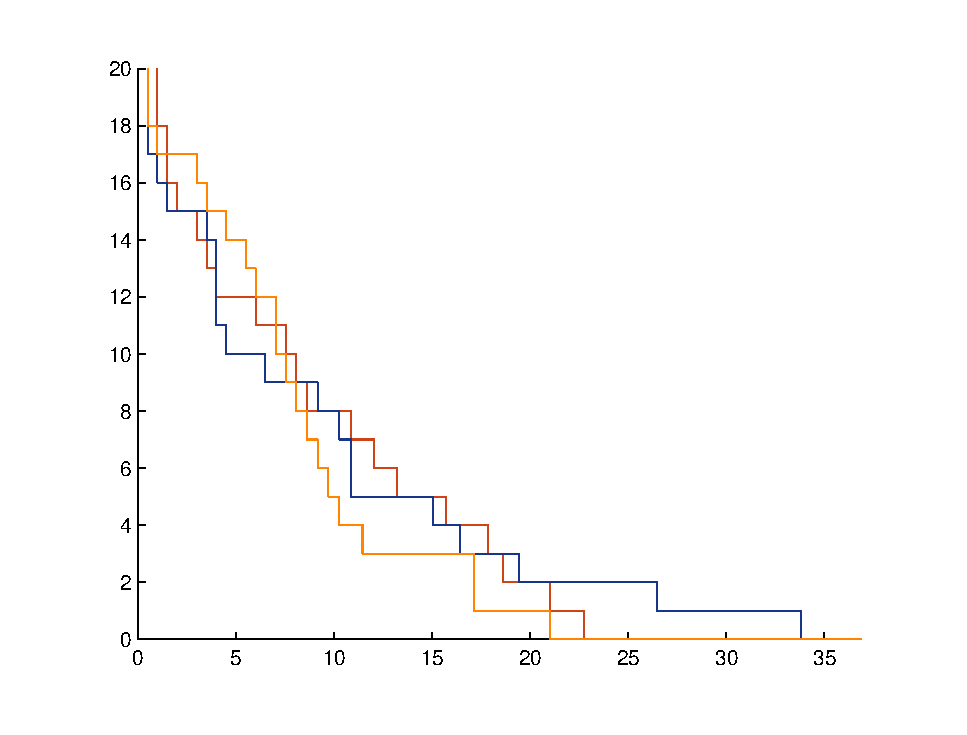
\includegraphics[width=\textwidth]{images/tau_decaying_individual.eps}
\caption{Three independent realizations of the simple degradation system \eqref{eq:simpledeg}. Parameterization: $k = 0.1$, $a(0) = 20$, $\epsilon = 0.05$}
\label{fig:tau_dec_indiv}
\end{figure}

\begin{figure}
\centering
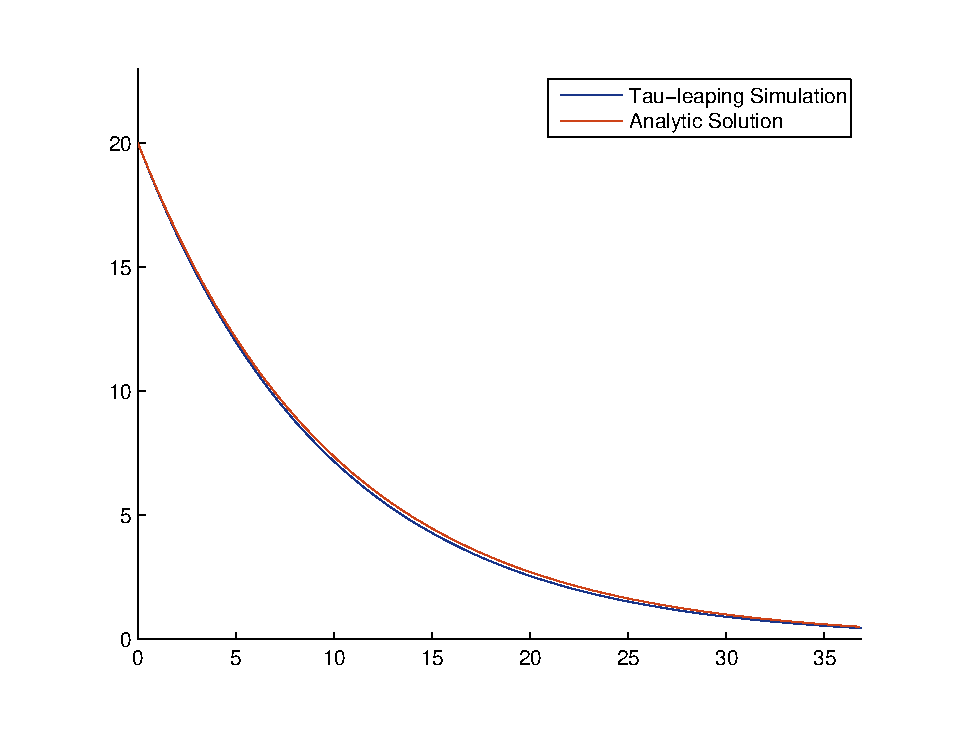
\includegraphics[width=\textwidth]{images/tau_decaying_average.eps}
\caption{Analytic solution of the simple degradation system \eqref{eq:simpledeg} and average of $128^3=2097152$ tau-leaping simulations. }
\label{fig:tau_dec_average}
\end{figure}


\paragraph{Production and degradation} Another system that is commonly used to validate stochastic simulation algorithms is the production-degradation system:

\begin{align}
\label{eq:gendeg1}
\cee{A &->[k_1] \emptyset{}} \\
\label{eq:gendeg2}
\cee{\emptyset{} &->[k_2] A}
\end{align}

For the reaction rates $k_1$ and $k_2$ values 0.1 and 1.0 are chosen, initial condition is $a(0) = 0$. Considering the two propensity functions $\alpha_1(t) = k_1 a(t)$ and $\alpha_2(t) = k_2$ it is trivial to see that the system is in equilibrium for $a=10$. The same observation can be made from the differential equation:
\begin{align}
\frac{da}{dt} = -k_1a+k2
\end{align}
The analytic solution is 
\begin{align}
a(t) = -10 \exp(-0.1t)+10
\end{align}

Figure \ref{fig:prod_deg_time} again shows a plot of the analytic solution and the average of ${128}^3$ tau-leaping simulations ($\epsilon = 0.05$). The maximum absolute error for $t \in [0,100]$ is 0.0525, the maximum relative error is 0.0525. In figure \ref{fig:prod_deg_hist} a histogram on the number of molecules at $t=100$ clearly shows the equilibrium for 10 particles. 

\begin{figure}
\centering
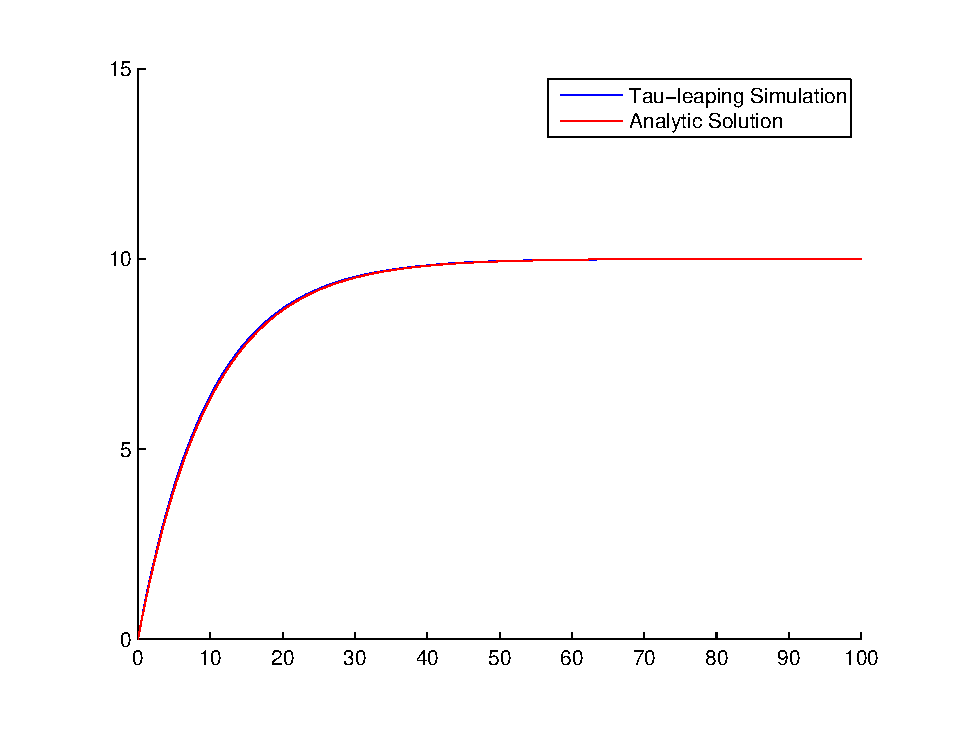
\includegraphics[width=\textwidth]{images/prod_deg_time.eps}
\caption{Analytic solution of the production-degradation system \eqref{eq:gendeg1}-\eqref{eq:gendeg2} and average of $128^3=2097152$ tau-leaping simulations. Parameterization: $k_1 = 0.1$, $k_2 = 1$, $a(0) = 0$, $\epsilon = 0.05$}
\label{fig:prod_deg_time}
\end{figure}

\begin{figure}
\centering
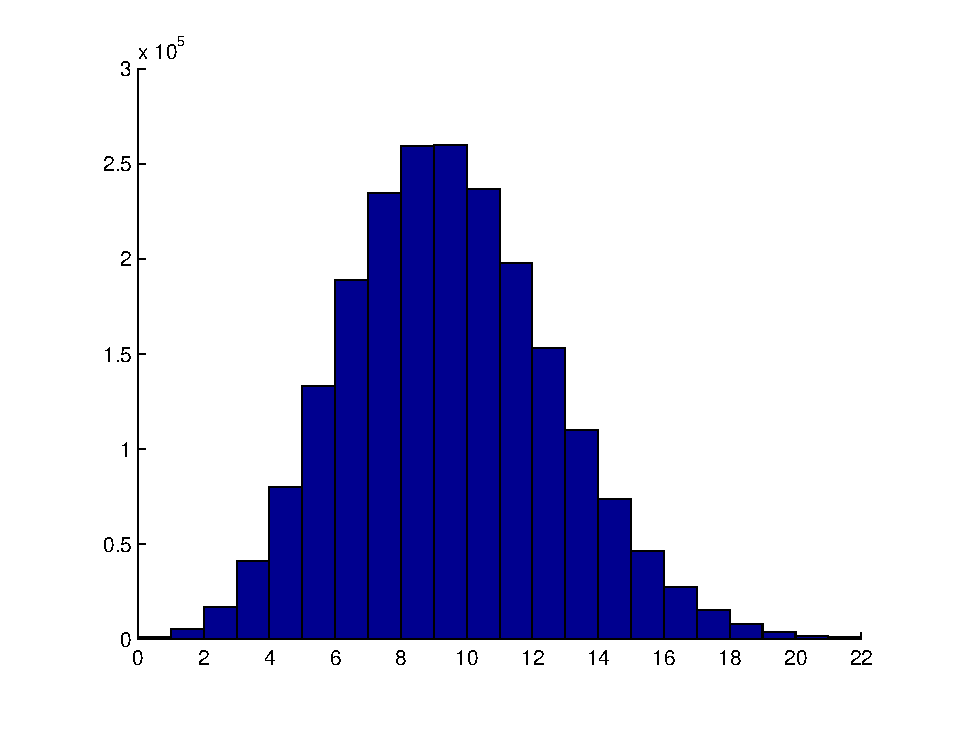
\includegraphics[width=\textwidth]{images/prod_deg_hist.eps}
\caption{Histogram of the production-degradation system \eqref{eq:gendeg1}-\eqref{eq:gendeg2}. Parameterization analogous to figure \ref{fig:prod_deg_time}. }
\label{fig:prod_deg_hist}
\end{figure}

\paragraph{2D heat equation} In order to validate the diffusion mechanism of the stochastic simulators the parabolic partial differential equation know as heat equation (in this context also called diffusion equation) is considered:
\begin{align}
\frac{\partial \rho(x,y,t)}{\partial t} = D \Delta \rho(x,y,t)=D\left(\frac{\partial^2 \rho(x,y,t)}{\partial x^2} + \frac{\partial^2 \rho(x,y,t)}{\partial y^2}\right)
\label{eq:heat}
\end{align}
$\rho(x,y,t)$ can either be considered the amount of heat or the concentration of some species at time $t$ in a point at $(x,y)$. The diffusion constant $D$ is a positive constant. To facilitate visualization two-dimensional diffusion is considered. 

The domain $\Omega$ shall be the unit square, i.e.} $x,y\in[0,1]$. The system is endowed with Dirichlet boundary conditions
\begin{align}
\rho(0,y,t)=\rho(x,0,t)=\rho(1,y,t)=\rho(x,1,t)=0 \;t>0
\label{eq:heatboundary}
\end{align}
and an initial distribution
\begin{align}
\rho(x,y,0) = \sin(x\pi) \cdot \sin(y\pi)
\label{eq:heatinit}
\end{align}

Under these conditions an analytic solution can be obtained:
\begin{align}
\rho(x,y,t) = \sin(x\pi= \cdot \sin(y\pi) \cdot \exp(-2\pi^2Dt)
\end{align}

Figures \ref{fig:diff_analytic} and \ref{fig:diff_stoch} show the state of the system ($D=10^{-3}$) at $t=60$ obtained by the analytic solution and tau-leaping stochastic simulation, respectively. For the latter 128x128 compartments, the accuracy control parameter $\epsilon = 0.05$ and the scaling constant $\Omega = 1000$ were used. 

The number of molecules is proportional to the volume integral over concentration. For the 2D case one has the following area integral: 
\begin{align}
C_{analytic} = \int_0^1 \int_0^1 \rho(x,y,60) = \frac{4}{\pi^2}\cdot \exp(-0.12\cdot \pi^2) \approx 0.12399
\end{align}
For the democratized stochastic approach it is equivalent to consider the sum over all compartments:
\begin{align}
C_{discrete} = \cdot \sum_{i,j} v_{i,j} \cdot \frac{x_{i,j}}{\Omega}
\end{align}
where $v$ is the volume of the compartment and $x$ the number of molecules in it. Considering the presented two-dimensional example with 128x128 uniform square-shaped compartments one has for the absolute error $\Delta C = \abs{C_{analytical} - C_{discrete}} \approx 1.4232\cdot10^{-5}$, for the relative error $\delta C = \Delta C / C_{analytic} \approx 1.1478\cdot 10^{-4}$.  

\begin{figure}
\centering
% l b r t
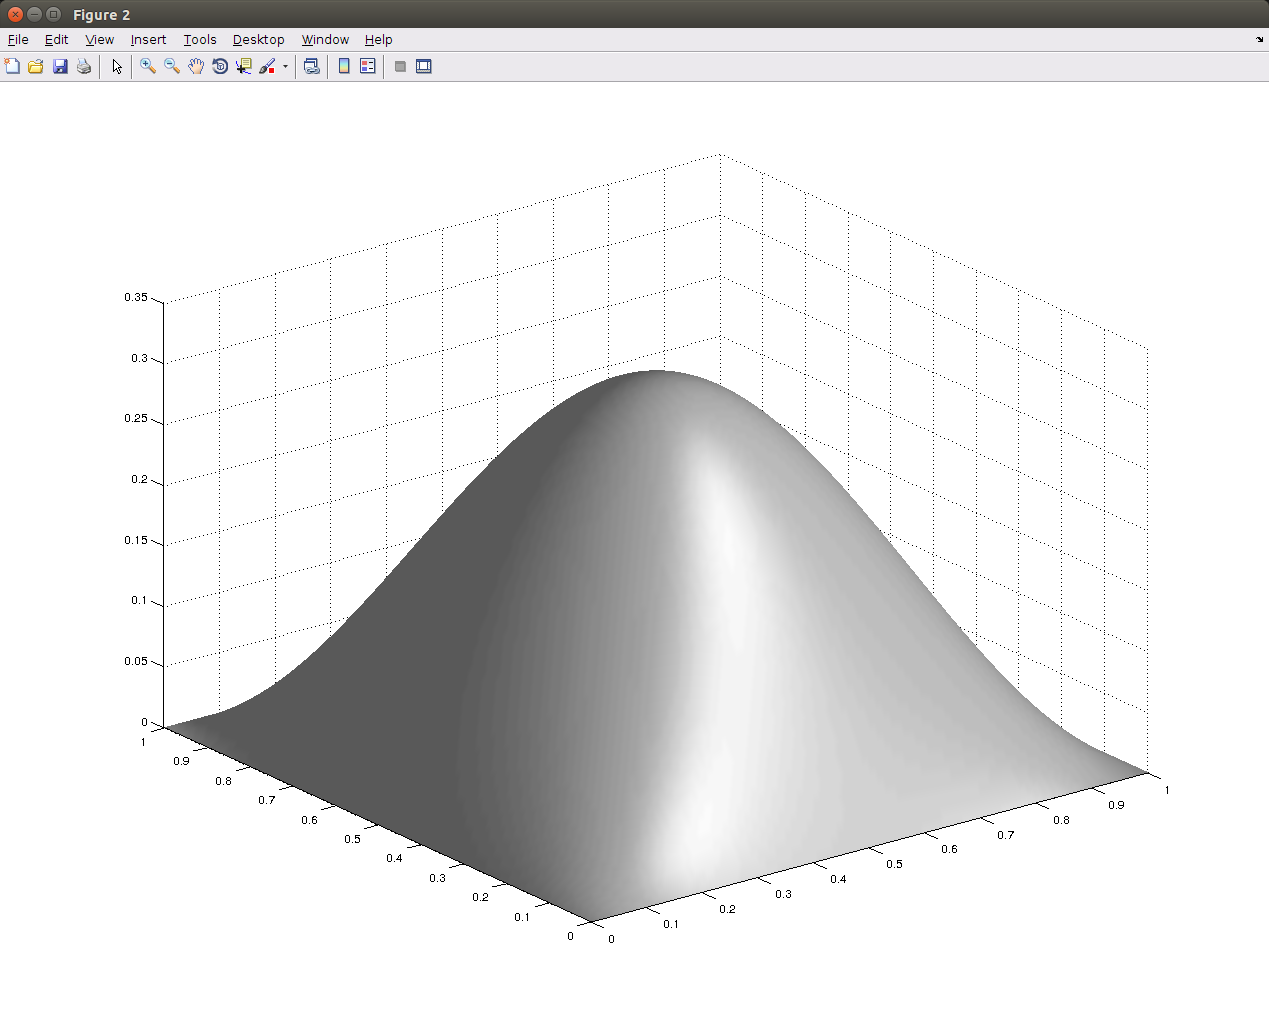
\includegraphics[trim = 15mm 0mm 10mm 35mm, clip, width=3cm,width=\textwidth]{images/diff_analytic.png}
\caption{Analytic solution of heat equation \eqref{eq:heat} for $D=10^{-3}$ with boundary condition \eqref{eq:heatboundary} and initial condition \eqref{eq:heatinit} at $t=60$.}
\label{fig:diff_analytic}
\end{figure}

\begin{figure}
\centering
% l b r t
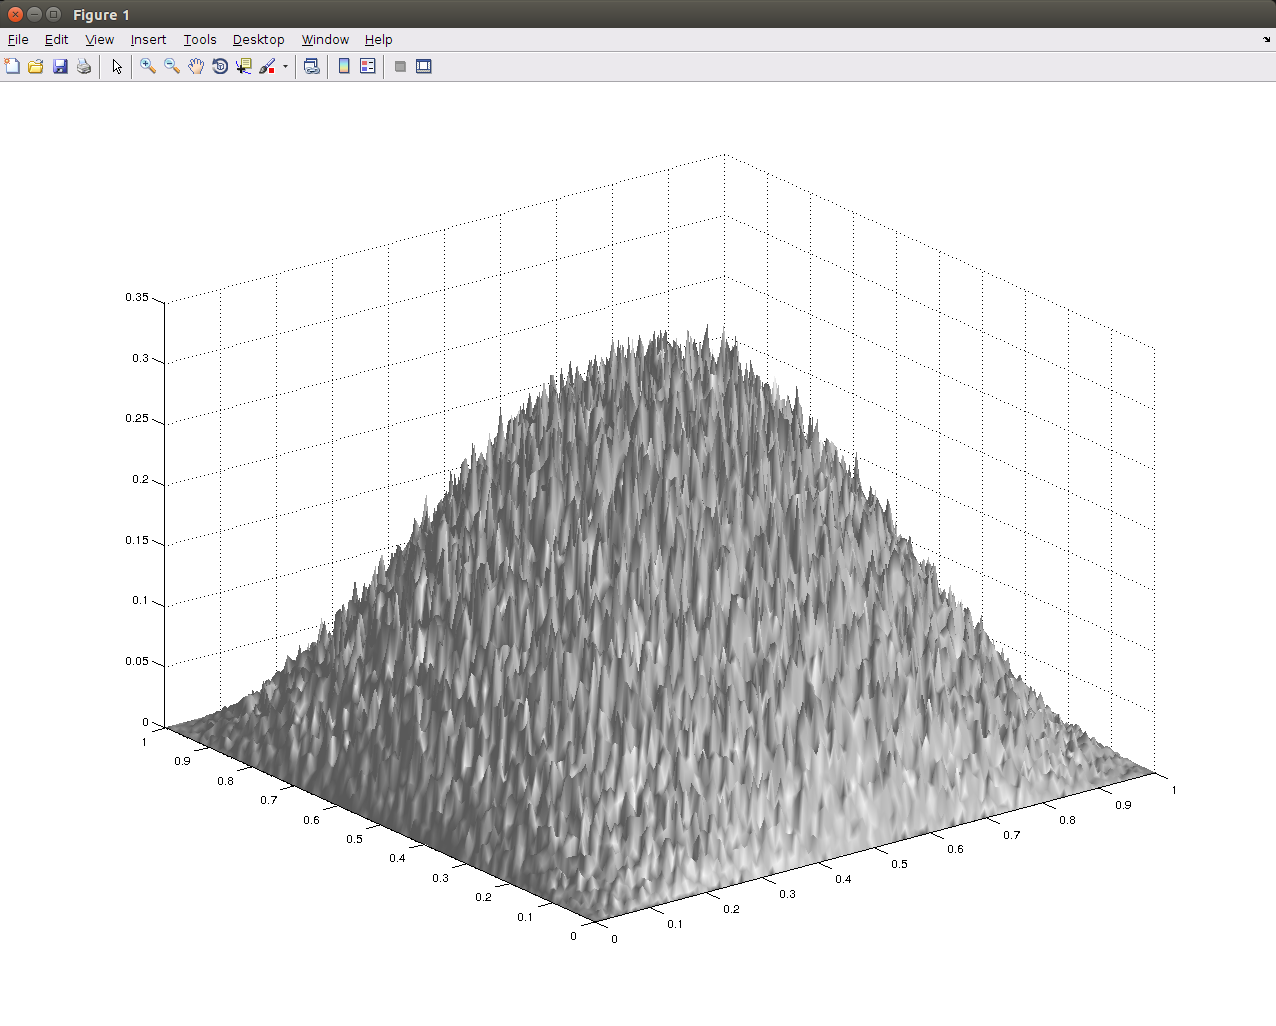
\includegraphics[trim = 15mm 0mm 10mm 35mm, clip, width=3cm,width=\textwidth]{images/diff_stoch.png}
\caption{Stochastic solution of heat equation \eqref{eq:heat} for $D=10^{-3}$ with boundary condition \eqref{eq:heatboundary} and initial condition \eqref{eq:heatinit} at $t=60$. Parameterization: $\epsilon = 0.05$, $\Omega = 1000$, spacing h=1/127}
\label{fig:diff_stoch}
\end{figure}


%\section{Pattern formation in the Gray-Scott System}
\section{Pattern formation in the Gray-Scott System}
One of the main reasons for the great interest in the Gray-Scott model is its ability to develop complex spatio-temporal patterns. Pattern formation is a form of self-organization which plays a central role in a variety of processes observed in nature that are crucial for the existence of live in any form (see chapter \ref{ch:intro} for examples). In this section it is shown how the developed stochastic simulator can be used to illustrate the temporal evolution of the system. 

The following initial conditions for the number of particles of species U and V are used throughout the whole thesis:
\begin{align}
 u_0 =
  \begin{cases} 
      \hfill    \Omega \left( \frac{1}{2} + \xi\cdot 10^{-2} \right) \hfill & \text{ if $\mathcal{G}_{int}$} \\
      \hfill \Omega \left( 1 + \xi \cdot 10^{-2} \right) \hfill & \text{ otherwise} \\
  \end{cases}
\end{align}
and
\begin{align}
 v_0 =
  \begin{cases} 
      \hfill    \Omega \left( \frac{1}{4} + \xi\cdot 10^{-2} \right) \hfill & \text{ if $\mathcal{G}_{int}$} \\
      \hfill \Omega \left( \xi \cdot 10^{-2} \right) \hfill & \text{ otherwise} \\
  \end{cases}
\end{align}
with random variable $\xi\! \sim\! \operatorname{Unif}(0,1)$ and inner region $\mathcal{G}_{int} = [1/4, 3/4]^d$ where $d$ is the dimension of the system under consideration. The initial conditions were chosen in dependence on \ref{rossinelli_accelerated_2008}. The parameters used are $F=0.04$, $\kappa = 0.06$, $\rho_d = 1-0$ (i.e.\ $\rho_s = 2.0$), $D_u = 2\cdot 10^{-4}$. 

Figure \ref{fig:pattern} illustrates the influence of the scaling parameter $\Omega$. For large values (e.g.\ $\Omega \gtrsim 10000$), the system is close to the thermodynamic limit, i.e.\ the deterministic approach is a valid approximation to the stochastic microscopic phenomena \ref{gillespie_deterministic_2009}. Figure \ref{todo} gives insight into the temporal evolution of the system, figure \ref{fig:3d} shows the isosurface for the concentration of species U at time $t=1000$ with respect to an isovalue of $0.5$. 

\begin{figure}
\centering
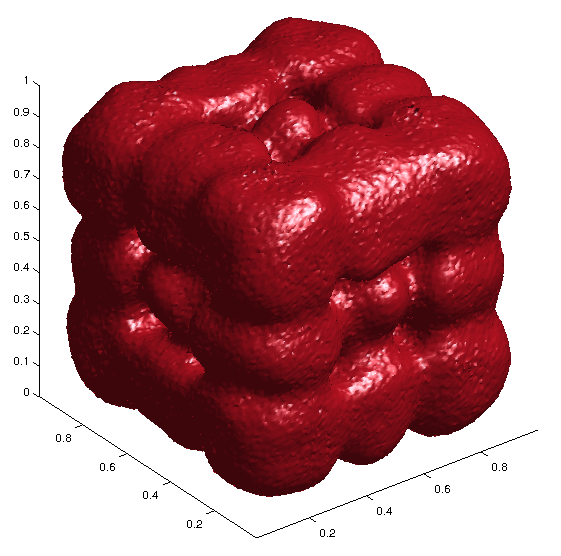
\includegraphics[height=0.4\paperheight]{images/3d.png}
\caption{Isosurface representation of the concentration of species U at $t=1000$ for an isovalue of 0.5.}
\label{fig:3d}
\end{figure}

In the literature and on the Internet numerous articles and websites on Gray-Scott pattern formation exist. Two especially illustrative resources on the topic shall be mentioned here: Project \textit{Xmorphia}\footnote{Original website unavailable. Extended version by R. Munafo: \url{http://goo.gl/vFnOU8}} by Roy Williams at Caltech and the \textit{Amorphous Computing}\footnote{\url{http://goo.gl/4iZUb1}} project by Abelson et al.\ at MIT CSAIL. Both websites enable interactive exploration of the system behaviour under different conditions. The former resource includes a map of the parameter space which directly links to videos that visualize the temporal evolution of the system for the selected setup. The latter includes interactive simulators and videos that illustrate the great variety of patterns that can be obtained. 

%Figure temporal evolution like previous

\begin{figure}
\centering
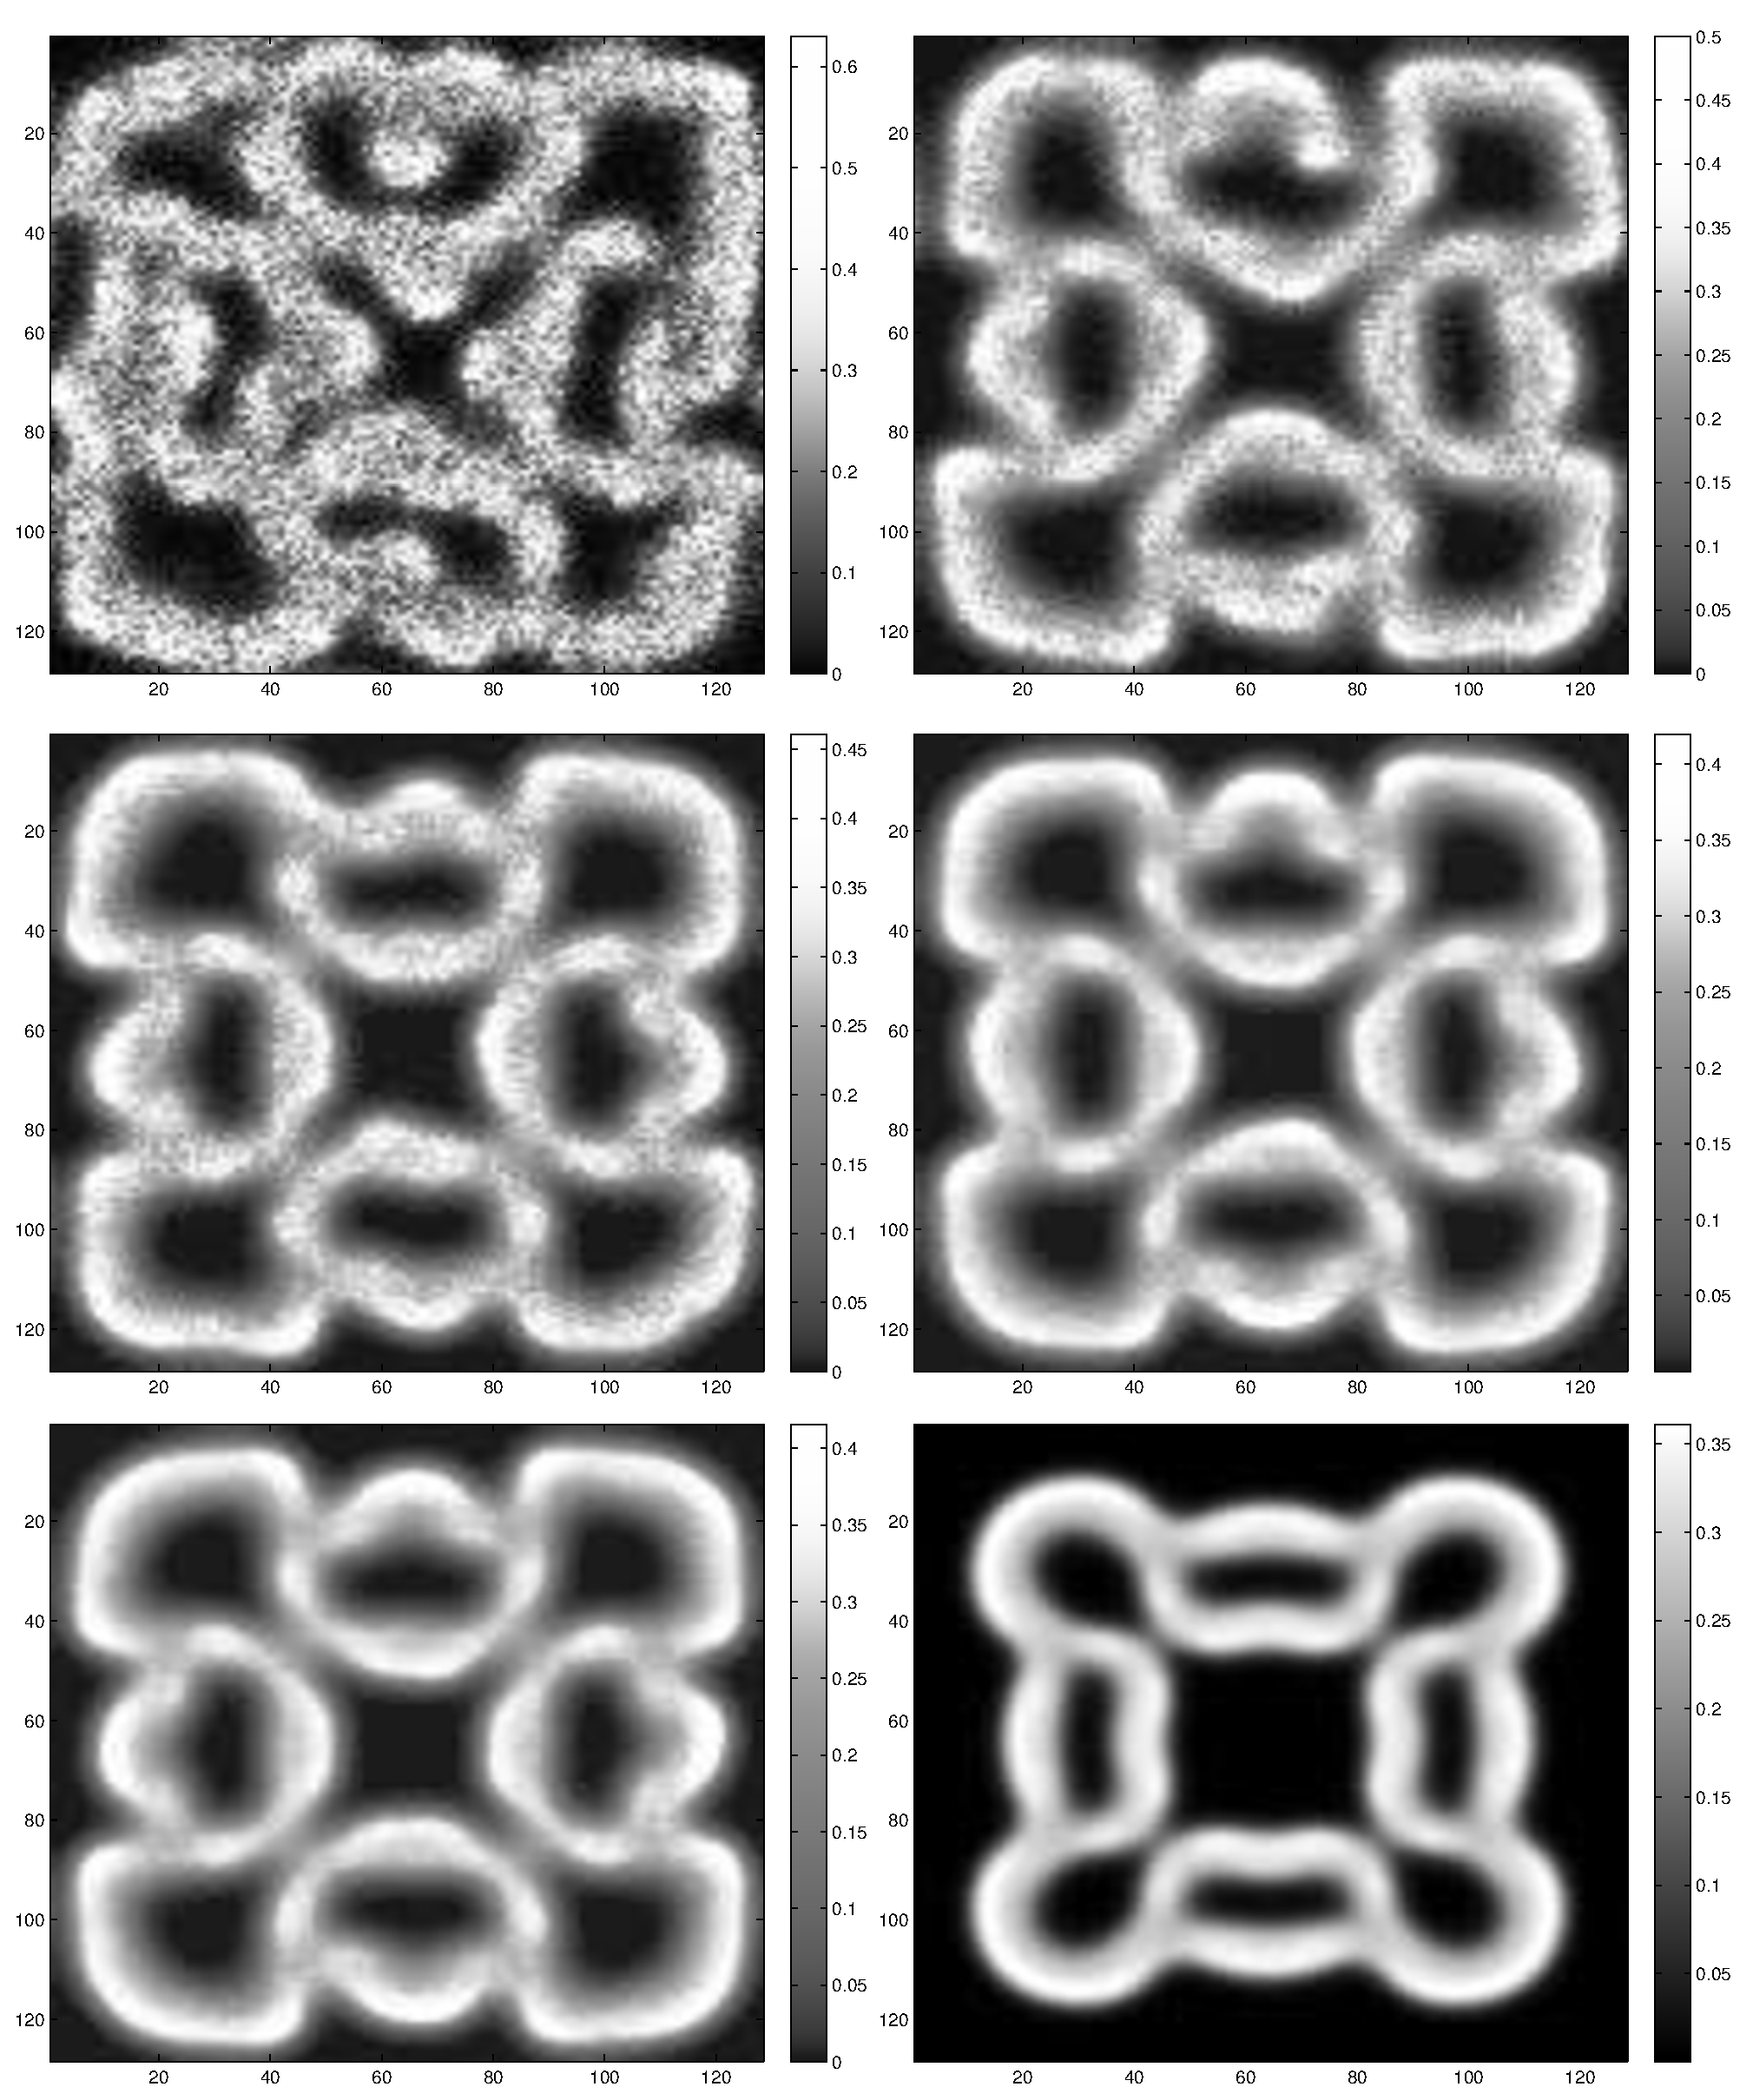
\includegraphics[width=\textwidth]{images/pattern.eps}
\caption{Pattern formation under the influence of varying molecule numbers. Figure shows simulation domain $[0,1]^3$ at time $t=1000$ divided in $128^3$ compartments and sliced at $x=0.6$. Parameters $F=0.04$, $\kappa = 0.06$, $\rho_d = 1-0$ (i.e.\ $\rho_s = 2.0$), $D_u = 2\cdot 10^{-4}$ and $D_v = 1\cdot 10^{-5}$ are used. From left to right and top to bottom the following values for $\Omega$ are used: 100, 500, 1000, 5000, 10000. The plot in the bottom right corner shows the deterministic solution (subject to finite-amplitude random perturbation) obtained with a finite difference approximation. Accuracy control parameter: $\epsilon = 0.05$}
\label{fig:pattern}
\end{figure}
%\section{Performance Analysis}
\section{Performance Analysis}
\label{ch:perf}
Simulation platforms: GTX 580, ...
% a9xxx : 3rd-generation nodes (2011) with 4 12-core AMD Opteron 6174 CPUs and InfiniBand network

\paragraph{Optimization of the GPU version} \label{ch:gpuopt} A GPU is a powerful but highly complex device. In order to ensure that an application uses the available resources efficiently performance evaluation and iterative optimization must be an integral part of the development process. The CUDA framework comes with advanced profiling tools (e.g.\ the Nvidia Visual Profiler) that automatically detect some of the worst pitfalls in GPU programming and can support the developer in trying to avoid them. 


In the following some optimization ideas that arouse during the development process of the GPU tau-leaping simulator are discussed. 

\begin{description}
\item[Initial] In chapter \ref{ch:gpuimplementation} three different approaches towards implementing diffusion were presented. In table \ref{tab:opti} execution times of one complete simulation step (i.e.\ tau calculation, reaction and diffusion) are given for each of the variants. As expected, the naive kernel performs worst since it does not used fast shared memory. The fact that \texttt{kernel\_shared} outperforms the more sophisticated alternative \texttt{kernel\_four}, on the other hand, might be surprising. In \ref{atomics} it has been shown that atomic operations on CUDA-enabled GPUs are significantly slower than regular memory transactions (up to 100x). In reality, however, it seems that the slowdown due to the overhead of three additional kernel launches and a more irregular access pattern overweights the benefits of avoiding atomics in global memory. The main reason for this result is definitely the accelerated hardware support for atomic operations in modern GPUs such as the Nvidia GeForce GTX 580 (in general compute capability $\geq$ 2.0). Another contributing factor is the small degree of the worst case collision, i.e.\ a maximum of four threads can possibly access a value in global memory at the same time. On GPUs it is often the case that a simple, computationally more expensive algorithm with simple control flow outperforms a complex, more efficient implementation that would be faster on a CPU. In the following only \texttt{kernel\_shared} is considered since it performed best in all stages of development and in the final simulator. 
\item[Combination of reaction and diffusion] As mentioned before the reaction and the diffusion operation can be merged. All information that is needed for simulating the local reactions is available within the diffusion kernel. Consequently the overhead of one kernel launch and more importantly several costly operations in global memory can be avoided. The relative speedup of this optimization is $\approx 4.3\%$. 
\item[Register count optimization] In chapter \ref{ch:gpuimplementation} the remark has been made that multiprocessor registers have to be considered a valuable resource in GPGPU computing. The reason will become obvious now: The original implementation of the reaction-diffusion kernel occupies 63 registers. Considering a block size of 512 threads (i.e.\ a 8x8x8 grid is used to reduce the number of global memory atomic operations) and 32768 registers that are available on each SM, only one block can reside on it at a time. This means that the number of threads that are available for execution in case a warp stalls to wait for a memory transaction is limited. As a result of the low \textit{occupancy} memory latency cannot be hidden by fast context switching. By using switches such as \texttt{-maxrregcount} the compiler can be forced to reduce the number of registers occupied by the kernel. Values that do not fit into registers any more are spilled to global memory. Trying to hide global memory latency by spilling variables to global memory may sound strange, but since heavily used values are kept in a on-chip L1 cache the approach is promising. By limiting the number of registers per thread to 31 two blocks can be scheduled per SM at the same time. The relative speedup obtained for the tau-leaping simulator is 11.2\%. 

It it obvious that the best alternative to forcing the compiler to lower register counts is not using a great number of registers in the first place. In a complex kernel such as the three-dimensional reaction-diffusion example where local as well as global boundary conditions and special cases have to be handled and comparably large PRNG states have to be kept in local memory reducing the number of registers is a nontrivial task. In future work together with improved compilers that apply more advanced optimization techniques based on compile time knowledge and control flow analysis a further increase in performance can be obtained. 

\item[Increase work per thread] Even in a framework such as CUDA that heavily relies on data parallelism a solution that exposes as much concurrent work as possible might not be the fastest. A good example for this optimization approach can be found in an example by Nvidia's Mark Harris \cite{nvidia reduction}. For the reaction-diffusion kernel under consideration it turns out that the average execution time of a simulation steps is minimized if every thread handles 16 compartments. This values has been obtained by heuristic experiments and depends on GPU generation and model. For the concrete example a considerable relative speedup of 39\% is achieved. 
\end{description}

\begin{table}[]
\centering
\newcolumntype{d}[1]{D{.}{\cdot}{#1} }
\begin{tabular}{|l|r|r|}
\hline
 \textbf{Optimization} & \textbf{Time / simulation step (ms)} & \textbf{Relative speedup}\\ \hline
 Initial (naive) & 21.98 & --- \mbox{     }\\ \hline
 Initial (shared) & 16.78 & --- \mbox{     }\\ \hline
 Initial (four) & 18.35 & --- \mbox{     }\\\hline
 Combination R\&D & 16.06 & 4.3\% \\ \hline
 Register count & 14.26 & 11.2\% \\ \hline
 Work per thread &  8.70 & 39.0\% \\ \hline
\end{tabular}
\caption{Execution time per simulation step and relative speedup of selected optimization steps. Absolute times are negatively affected by the performance measurement itself since additional synchronization is needed. Values obtained during the standard 128x128x128 compartment simulation of the Gray-Scott model. }
\label{tab:opti}
\end{table}

\paragraph{Optimization of the CPU version} Due to the rather coarse grained task parallelism approach of OpenMP optimizing methods for the CPU version are limited. Avoiding the overhead of one fork-join operation per step by introducing one large parallel region reduces the execution time per step by approximately 50\% (1.05s vs.\ 0.54s on an Intel Core i5-2430M with four threads\ref{todo check consistency}). Further optimization techniques may involve the use of vector instructions (SSE, AVX) or the introduction of cache-optimized access patterns (tiling, space-filling curve). Those techniques are highly complex to implement and far beyond scope. In this thesis the potential of two parallel platforms for accelerating stochastic simulations in time-limited academic projects is assessed. In this framework an optimal solution in terms of efficiency is neither possible to achieve nor a necessity. 

\paragraph{GPU strong domainsize} Medium sized system: performance leader \\
by no means perfect: peak throughput: schoenrechnen \\

\paragraph{CPU scaling number of threads} Memory limited and scaling

\paragraph{resume} Difference factor. But in reality highly optimized version. CUDA forces developer to vectorize, makes it easy. 

\ifdebug
1. 1 second simulation of tau leaping cpu 1-48 threads and naive, chessboard
2. GPU optimization steps
3. gpu scaling: size of system
3. same system



\begin{itemize}
\item Cite 'Debunking ...'
\item Speedup GPU vs.\ CPU
\item Bandwith vs. theoretical
\item Ideas to optimize
\end{itemize}
Simulation Performance?
\begin{itemize}
\item deviceQuery GTX 580 (global memory: 1535 MB, 16 SM, 32 CC/SM, GPU clock 1,62 GHz, Memory CR 2016 MHz, M Bus Width 384-bit, Smem / block: 49152 bytes, registers per block 32768, tpb 1024, tpSM 1536)
\item Time per step
\item Time to solution
\item Bandwidth estimation
\item FLOP/s from cuvpp?
\item Optimizations: Approaches to diffusion
\item Occupancy: PTX, ...
\item Several cells per block
\item GPU outperforms CPU by a factor of 25x to 100x (Nobile)
\end{itemize}

\ifdebug
Optimization: Reduce # register -> occupancy -> hide latency
\fi

\ifdebug
\section{Comparison of of both systems and implications on implementation strategies}
fields of application

\begin{itemize}
\item No complex memory hierarchy
\item Tiling is natural on GPU
\item ...
\item data level parallelism vs.\ thread parallelism
\end{itemize}
rule of thumb: complex control flow: cpu, simple control view, parallelizable, vectorization, data centric
\fi
\fi